% This is a sample file for submission of your preprint to Peer Community In (PCI) for evaluation or for transfer of your PCI-recommended article to Peer Community Journal (PCJ) for publication. 
%
%To submit to PCI for evaluation, you have to prepare a pdf file of all the contents pages of your paper, including the cover page: this behavior is triggered by removing the class option 'mode=plain' below.
%
%To transfer your PCI-recommended article to PCJ for publication, you have to prepare a pdf file without the cover page and header/footers: this behavior is triggered by the class option 'mode=plain' below. The cover page, including the metadata, the abstract, and the page headers/footers will be added upon online publication by the admin staff of the journal.
%
% This "author package" does not contain all the files necessary to support typesetting of a PCJ cover page. The cover page, including the metadata, the abstract, and the page headers/footers will be added upon online publication by the admin staff of the journal.

% add 'mode=plain' to transfer to PCJ
% remove 'mode=plain' to submit to PCI
\documentclass[PCJ,Unicode,screen]{cedram}

\usepackage[
natbib=true,
mincitenames=1,
maxcitenames=2,
maxbibnames=20,
minbibnames=20,
uniquelist=false,
uniquename=false,
style=pcj
]{biblatex}
\usepackage{lipsum}
\usepackage{setspace}

% This is to correct wrong references sorting, see sample .bib file.
\providecommand*{\noopsort}[1]{}

% To suppress unwanted field in the bibliography:
\AtEveryBibitem{%
  \iffieldundef{doi}{}{%
  \clearfield{url}%
  \clearfield{urldate}%
  }%
  \clearfield{note}%
  \clearfield{publisher}%
  \clearfield{isbn}%
  \clearfield{issn}%
}

%%%%%%%%%%%%%%%%%%%%%%%%%%%%%%%%%%%%%%%%%%%%%%%%%%%%%%%%%%%%%
% Declare your BibTeX file here (keep the .bib extension):
\addbibresource{PCJ-sample.bib}

% Article metadata: these are useless when transferring your article to PCJ because they only appear on the cover page and article headers/footers after publication, and you are not asked/expected to generate these elements (there is a separate web interface to fill them in during the submission process).

\DOI{10.5802/fake.doi} % this is the DOI of the preprint on the preprint server
\PCIcorresp{machin@example.edu}

\title[Sample for the template]{Sample for the template, with quite a very long title}
%
 \author{\firstname{Antoine} \lastname{Lavoisier}\IsEqualContrib}
 \address{Rue sans aplomb, Paris, France}
 \email[A. Lavoisier]{a-lavois@lead-free-univ.edu}
%
 \author{\firstname{Mary} \middlename{P.} \lastname{Curry}\IsEqualContrib}
 \address{Center for spiced radium experiments, United Kingdom}
 \email[M.~P.~Curry]{m.p.curry@radexp.edu.uk}
%
 \author{\firstname{Dick} \lastname{Darlington}}
 \address{Bruce's Bar and Grill, London (near Susan's)}
 \email[D.~Darlington]{dd@example.com}
%
 \author{\firstname{Peter} \lastname{Curry}}
 \address{Center for spiced radium experiments, United Kingdom}
 \email[P.~Curry]{p.curry@radexp.edu.uk}

 \keywords{Example, Keyword}
%
 \begin{abstract}
     \lipsum[1]
 \end{abstract}
%
%%%%%%%%%%%%%%%%%%%%%%%%%%%%%%%%%%%%%%%%%%%%%%%%%%%%%%%%%%%%%%%%%%%%%%%%%%

\begin{document}

\maketitle
%you may choose to use a table of content
%\tableofcontents
\onehalfspacing
\section*{Example of a section, e.g. Introduction}
\lipsum[3]
\section*{Example of a section, e.g. Material and methods }
\lipsum[4]
\subsection*{First subsection}
\lipsum[5]
\subsection*{Second subsection}
\lipsum[6]
\subsection*{Third subsection}
\lipsum[7]
\section*{Example of a section, e.g. Results }
\lipsum[8]
\begin{landscape}
    \section*{Landscape section}
    \lipsum[9-11]
\end{landscape}

\section*{Example of a section, e.g. Discussion}
\lipsum[12]
\begin{itemize}
\item toto (see Appendix~\ref{sA} and Eq.~\ref{eq:eq1})
\item foo (see Figure~\ref{fig:fig1})
\item bar
\end{itemize}

\subsection*{An other subsection}
\lipsum[13]
\begin{enumerate}
\item first item
\item second item
\begin{enumerate}
\item \label{2a} item \ref{2a}
\item item 2b (cf.~\cite[Thm.~3]{Ivanov_curve-complex_1997})
\end{enumerate}
\end{enumerate}

\subsubsection*{A subsubsection}
\lipsum[14]
\\This is an equation:

\begin{equation}
1=1
\label{eq:eq1}
\end{equation}

\paragraph{A paragraph}
\lipsum[15]

\subparagraph{A subparagraph}
Not much difference with a regular \verb+\paragraph+ \parencite{fake}.
\lipsum[16]

\begin{multline}
\exp(x) = 1 + x + \frac{x^2}{2!} + \frac{x^3}{3!} + \frac{x^4}{4!} + \frac{x^5}{5!} + \frac{x^6}{6!} + \frac{x^7}{7!} + \frac{x^8}{8!} + \frac{x^9}{9!}\\
\\+ \frac{x^{10}}{10!} + \frac{x^{11}}{11!} + \frac{x^{12}}{12!} + \frac{x^{13}}{13!} + \frac{x^{14}}{14!} + \frac{x^{15}}{15!} + \frac{x^{16}}{16!} + o(n^{16}).
\end{multline}

\begin{figure}[ht]
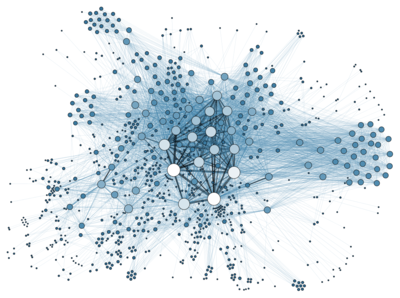
\includegraphics[scale=0.5]{pci-graph-small.png}
\caption{This is the title of the figure. It also contains the legend of the figure, with some math to check everything is working: $\log(\frac12)$. The caption is different from the caption of the table (see table~\ref{tab:tab1})}
\label{fig:fig1}
\end{figure}

\lipsum[19]

\begin{table}[ht]
\caption{This is the title of the table. It also contains the legend i.e. an explanation of what the table reveals about the problem at hand (typeset using \texttt{\textbackslash caption}).}
\begin{tabular}{rcccc}
    \hline &&&&\\[-0.95em]
    $n$&1&2&3&4\\ \hline &&&&\\[-0.95em]
    $n^2$&1&4&9&16\\ &&&&\\[-0.95em]
    $n^3$&1&4&9&18\\ \hline  &&&&\\[-0.95em]
\end{tabular}
\caption*{This is the note of the table if required. It is below the table to look nice. This can be done by using the command \texttt{\textbackslash caption*}. Compare with the figure caption above (see Figure~\ref{fig:fig1}).}
\label{tab:tab1}
\end{table}

\begin{proof}
This is a proof that ends with a \verb+{align}+ type of equation. The last equation should be numbered, but \verb+\qedhere+ breaks it (yet it works in most other journals?)
\begin{align}
&1234596748613548534863\\
&bjklbjl\\
&1234864 + \sum_{i=1}^{n}\frac{1}{i}\qedhere
\end{align}
\end{proof}

\section*{Example of a section, e.g. Conclusion}
\lipsum[20]

\appendix
\section{Some other things}\label{sA}
If your appendices fit in less than 2 pages, add your appendices here.

If your appendices take more than 2 pages, please proceed as follows:
\begin{itemize}
\item deposit them in an open repository such as Zenodo
\item add the DOI and the citation in the section “Data, scripts, code, and supplementary information availability”
\item add the reference in the list of references
\end{itemize}

\section*{Acknowledgements}

This is your acknowledgments. Preprint version xxx[change to the correct number] of this article has been peer-reviewed and recommended by Peer Community In XYZ[change to the name of the PCI] (\url{https://doi.org/10.24072/pci.xxx}[replace by the doi of the
recommendation]; \cite{fake}[replace by the citation of the recommendation]).


\section*{Fundings}

Declare your fundings. If your study has not been supported by particular
funding, please indicate ``The authors declare that they have received no
specific funding for this study''.

\section*{Conflict of interest disclosure}

The authors declare that they comply with the PCI rule of having no financial conflicts of interest in relation to the content of the article. [IF APPROPRIATE: The authors declare the following non-financial conflict of interest: XXX (if some of the authors are recommenders of a PCI, indicate it here)].

\section*{Data, script, code, and supplementary information availability}

Data are available online (\url{https://doi.org/10.24072/fake1}[Replace by the DOI of the webpage hosting the data]; \cite{CharleMar_independant-trace-su2_2012}[Replace by the citation of the data])\\
Script and codes are available online (\url{https://doi.org/10.24072/fake2}[Replace by the DOI of the webpage hosting the script and code]; \cite{CharleMar_independant-trace-su2_2012}[Replace by the citation of the script and code])\\
Supplementary information is available online (\url{https://doi.org/10.24072/fake3}[Replace by the DOI of the webpage hosting the Supplementary information]; \cite{CharleMar_independant-trace-su2_2012}[Replace by the citation of the Supplementary information])\\ \\
The DOI hyperlinks should be active. They should also be present in the reference list and cited in the text.
\\For the reference section below, do not forget to add a doi for each reference (if available). Do not forget to add the reference of the recommendation, the reference of the data, scripts, code and supplementary material to your bib file, if appropriate.

\printbibliography
\end{document}
